%-*- coding: UTF-8 -*-
\documentclass[UTF8]{ctexart}
\usepackage{geometry}
\geometry{a4paper,centering,scale=0.8}
\usepackage{graphicx}
\usepackage{amsmath}
\usepackage{textcomp}
\usepackage{amsthm}
\usepackage{amssymb}
\usepackage{float}

\title{\heiti Deep Learning}
\author{卢婧宇}

\begin{document}
\maketitle
\tableofcontents

\newpage
\section {Neural Networks \& Deep Learning 神经网络和深度学习}
\subsection{Building your Deep Neural Network: Step by Step(第四周作业)}
\subsubsection{Outline of the Assignment}
\begin{itemize}
  \item 双隐藏层和L层神经网络模型的参数初始化
  \item 做前向传播
  \begin{itemize}
    \item 计算正向传播的LINEAR 部分,
    线性部分即Z=WX+b这部分,输出部分就是A,就是将线性部分的结果输入到激活函数所产生的结果。
    \item 采用RELU或者sigmoid激活函数计算结果值
    \item 联合上述两个步骤,进行前向传播操作[LINEAR->ACTIVATION]
    \item 对输出层之前的L-1层,做L-1次的前向传播 [LINEAR->RELU] ,并将结果输出到第L层[LINEAR->SIGMOID]。所以在前面L-1层的激活函数是RELU,在输出层的激活函数是sigmoid。
  \end{itemize}
  \item 计算损失函数
  \item 做后向传播操作
  \begin{itemize}
    \item 计算神经网络反向传播的LINEAR部分
    \item 计算激活函数(RELU或者sigmoid)的梯度
    \item 结合前面两个步骤,产生一个新的后向函数[LINEAR->ACTIVATION]
  \end{itemize}
  \item 更新参数
\end{itemize}

\begin{figure}[htb]
 \center{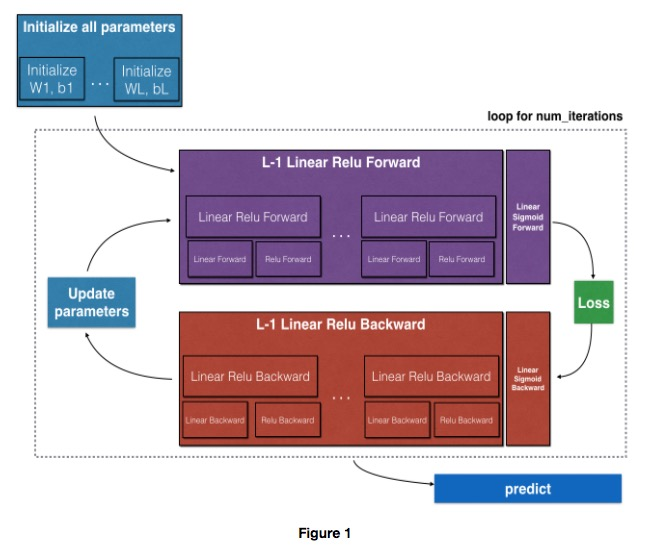
\includegraphics[width=8cm]  {1.jpg}}
 \caption{流程图}
 \label{fig:1}
 \end{figure}

\subsubsection{L-layer Neural Network}
对于L层模型:
\begin{itemize}
  \item 模型结构: [LINEAR -> RELU] × (L-1) -> LINEAR -> SIGMOID。所以 L−1 层是需要用到 ReLU激活函数的。输出层用的是sigmoid函数。
\item 权重矩阵采用仍旧是随机化初始化的方式: np.random.rand(shape) * 0.01
\item 偏移矩阵仍旧是0矩阵进行处初始化: np.zeros(shape).
\item 我们将每层的神经元数量n[l]信息进行存储,layer\_dims。例如在平面数据分类模型中 layer\_dims 的值是[2,4,1],其中输入层的神经元个数是2,
  隐藏层的神经元个数是4,输出层的神经元个数是1。对应的 W1尺寸= (4,2), b1尺寸= (4,1), W2尺寸= (1,4) , b2 尺寸= (1,1)。
\end{itemize}

GRADED FUNCTION: initialize\_parameters\_deep
\begin{figure}[htb]
 \center{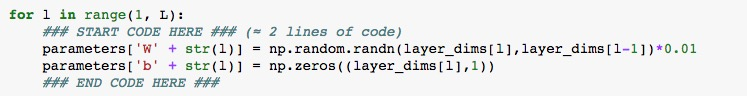
\includegraphics[width=11cm]  {2.jpg}}
 \caption{初始化W,b}
 \label{fig:2}
 \end{figure}

\subsubsection{Forward propagation module}
线性传播部分:

GRADED FUNCTION: linear\_forward
 \begin{figure}[htb]
  \center{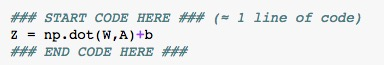
\includegraphics[width=8cm]  {3.jpg}}
  \caption{Z的计算}
  \label{fig:3}
  \end{figure}

激活部分:

运用两个激活函数:

Sigmoid.在这个步骤我们需要两个结果,一个是激活函数的结果值,另一个是包含``Z''的``cache''值 ,这个我们在后向传播过程需要用到。
     A, activation\_cache = sigmoid(Z)

ReLU.A=RELU(Z)=max(0,Z).同样结果值有两部分,其一是激活函数结果值``A'' ,另一个是包含``Z''的 ``cache''值。
   A, activation\_cache = relu(Z)

(a)相邻两层的激活实现

GRADED FUNCTION: linear\_activation\_forward
   \begin{figure}[htb]
    \center{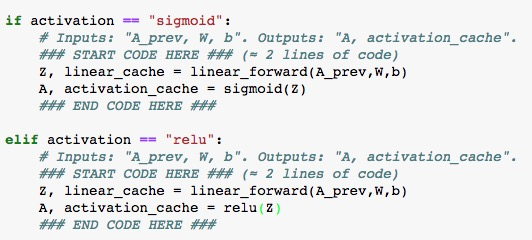
\includegraphics[width=10cm]  {4.jpg}}
    \caption{激活函数}
    \label{fig:4}
    \end{figure}

\newpage
(b)L-Layer Model (L 层模型)

那么对于L层的神经网络,激活函数为RELU的linear\_activation\_forward 需要重复L-1次,而最后的输出层采用的参数为SIGMOID的linear\_activation\_forward 。

GRADED FUNCTION: L\_model\_forward

[LINEAR -> RELU] × (L-1) -> LINEAR -> SIGMOID model

\begin{figure}[htb]
 \center{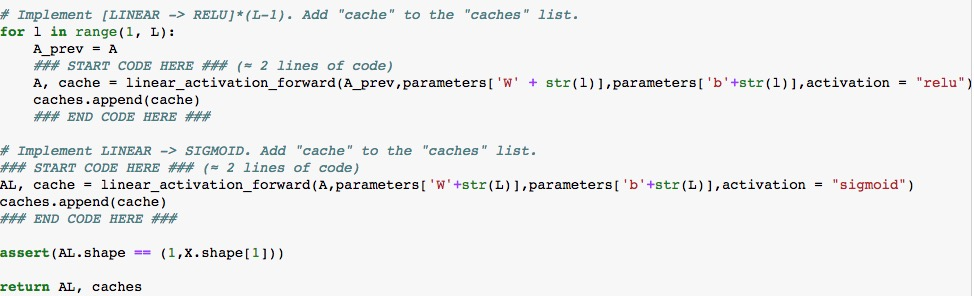
\includegraphics[width=12cm]  {5.jpg}}
 \caption{L层前向传播}
 \label{fig:5}
 \end{figure}

 \subsubsection{Cost function}
 \begin{figure}[htb]
  \center{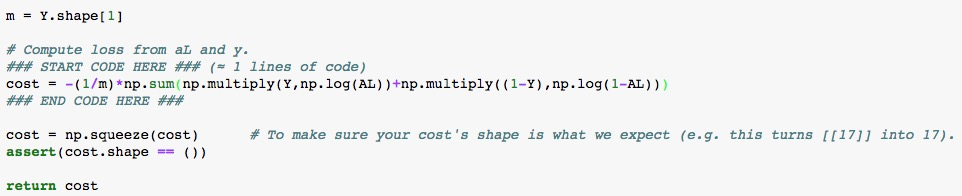
\includegraphics[width=12cm]  {6.jpg}}
  \caption{代价函数}
  \label{fig:6}
  \end{figure}

\subsubsection{Backward propagation module}
后向传播是为了计算各个参数梯度,其模型如下:

\newpage

\begin{figure}[htb]
 \center{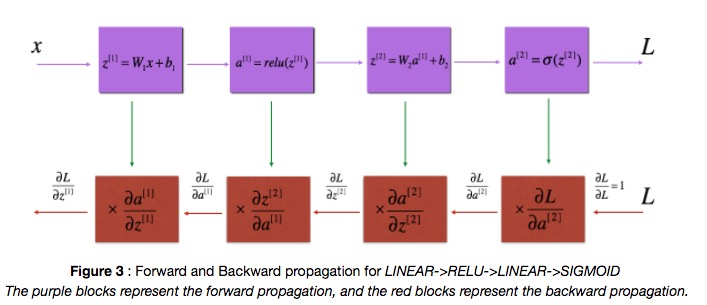
\includegraphics[width=10cm]  {7.jpg}}
 \caption{后向传播}
 \label{fig:7}
 \end{figure}


 和之前的前向传播类似,后向传播模块的建立分以下三个步骤:
\begin{itemize}
  \item 后向LINEAR(Linear backward)
  \item ReLU 或者 sigmoid 激活函数的后向LINEAR -> ACTIVATION
  \item $[$LINEAR -> RELU$]$× (L-1) -> LINEAR -> SIGMOID backward (whole model)
\end{itemize}

 后向Linear

 三个输出 ($dW^{[l]},db^{[l]},dA^{[l]}$) 可以通过输入$dZ^{[l]}$计算获得。公式如下:
 \begin{figure}[htb]
  \center{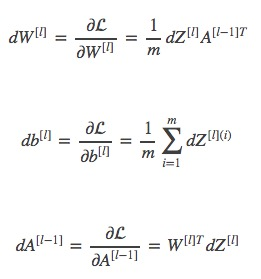
\includegraphics[width=4cm]  {8.jpg}}
  \caption{后向传播公式}
  \label{fig:8}
  \end{figure}

GRADED FUNCTION: linear\_backward
\begin{figure}[htb]
 \center{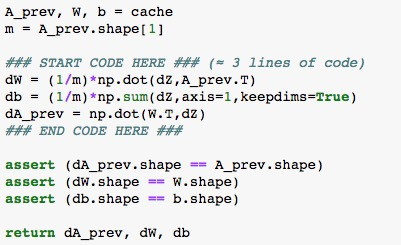
\includegraphics[width=8cm]  {9.jpg}}
 \caption{后向传播公式}
 \label{fig:9}
 \end{figure}

(a)Linear-Activation backward

对于sigmoid函数,可以定义两个函数:

sigmoid\_backward:用以计算 SIGMOID单元:dZ = sigmoid\_backward(dA, activation\_cache) 其用到的cache值是Z值

relu\_backward: 用以计算RELU的 backward propagation:dZ = relu\_backward(dA, activation\_cache)

对于 g(.)的激活函数:

sigmoid\_backward 和relu\_backward 的计算如下:$dZ^{[l]}=dA^{[l]}*g^{'}(Z^{[l]})$

GRADED FUNCTION: linear\_activation\_backward
\begin{figure}[htb]
 \center{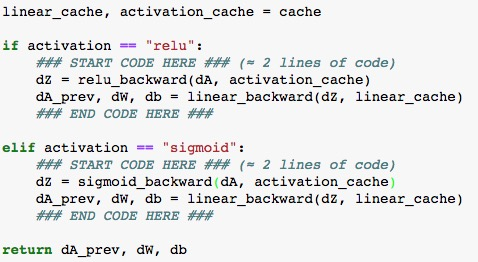
\includegraphics[width=8cm]  {10.jpg}}
 \caption{线性激活函数反向传播}
 \label{fig:10}
 \end{figure}

 (b)L-Model Backward

对整个神经网络做后向传播,定义函数为L\_model\_forward。在每次的迭代过程中,
我们都将 cache值=(X,W,b, z)保留,用以后向模块中梯度的计算。在L\_model\_forward中,我们是重复了L次上述的步骤。
\begin{figure}[htb]
 \center{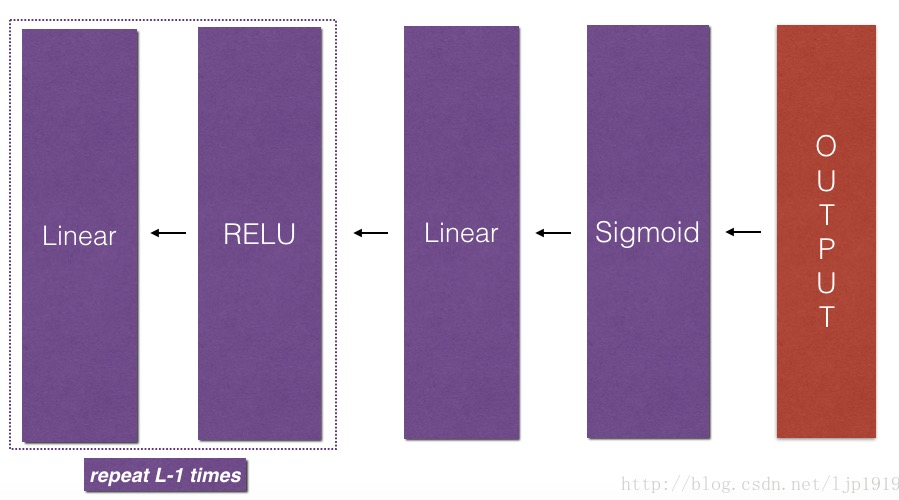
\includegraphics[width=8cm]  {11.jpg}}
 \caption{L层反向传播}
 \label{fig:11}
 \end{figure}

 后向传播初始化:

 对于后向传播,我们知道前向传播的输出是$A^{[L]}=\sigma (Z^{[L]})$,我们需要计算 $dAL=\frac{\partial L}{\partial A^{[L]}}$,
 我们用以下的公式表示:
 dAL = - (np.divide(Y, AL) - np.divide(1 - Y, 1 - AL)) derivative of cost with respect to AL

 之后,我们可以用这个后向激活的梯度 dAL 进行向后传播。再从 dAL 计算 LINEAR->SIGMOID 的后向传播结果。对于 LINEAR->RELU backward 函数,
 我们可以采用for 循环来处理这L-1次操作。在此期间,我们要存储 dA, dW, db,本文用grads字典来存储:
 $grads[``dW''+str(l)]=dW^{[l]}$

 例如, 对于l=3,则 $dW^{[l]}$ 以 grads[``dW3'']形式存储。

 模型如下:
 [LINEAR->RELU] × (L-1) -> LINEAR -> SIGMOID

GRADED FUNCTION: L\_model\_backward
\begin{figure}[htb]
 \center{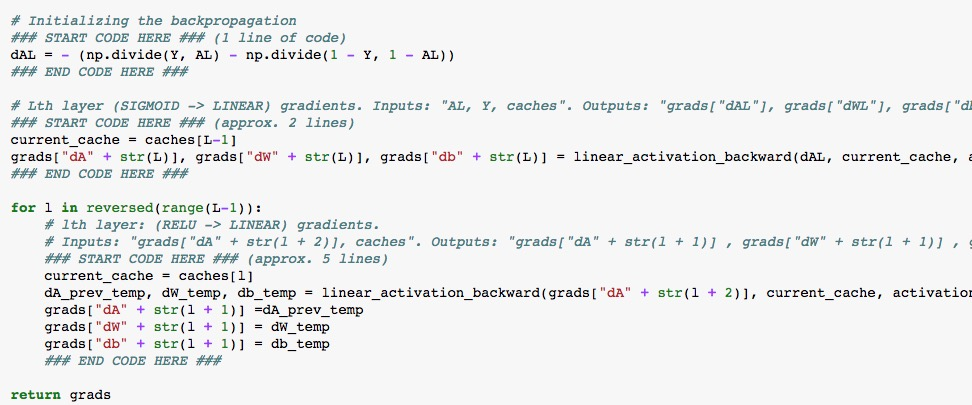
\includegraphics[width=12cm]  {12.jpg}}
 \caption{L层反向传播模型}
  \label{fig:12}
 \end{figure}

 Update Parameters

 采用梯度下降进行参数的更新:$W^{[l]}=W^{[l]}−\alpha dW^{[l]}$ $ b^{[l]}=b^{[l]}−\alpha db^{[l]}$
 \begin{figure}[htb]
  \center{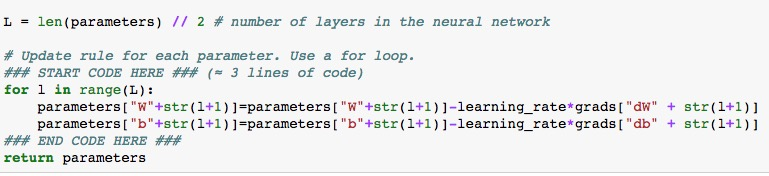
\includegraphics[width=12cm]  {13.jpg}}
  \caption{更新}
   \label{fig:13}
  \end{figure}

  \subsubsection{General methodogy 通用模型}
  As usual you will follow the Deep Learning methodology to build the model:
  \begin{itemize}
    \item Initialize parameters / Define hyperparameters
    \item Loop for num\_iterations:
    \begin{itemize}
      \item Forward propagation
      \item Compute cost function
      \item Backward propagation
      \item Update parameters (using parameters, and grads from backprop)
    \end{itemize}
    \item Use trained parameters to predict labels
  \end{itemize}
lement those two models!

\section{Improve Deep Neural Networks}
\subsection{Initialization}
一个好的初始化参数能够加速梯度下降的收敛,同时能够以较大几率使得梯度下降收敛到较低的训练(和泛化)误差。
\subsubsection{Zero initialization 全零初始化 }
 parameters = initialize\_parameters\_zeros(layers\_dims)
 \begin{figure}[htb]
  \center{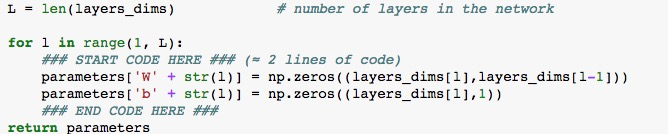
\includegraphics[width=10cm]  {14.jpg}}
  \caption{全零初始化}
   \label{fig:14}
  \end{figure}

效果很差,整个迭代过程损失函数并没有下降。该参数下的模型对于训练集和测试集的预测结果全为0。

该模型预测结果是没有边界的,因为都是预测结果都是一类,都是0。
这种全0的参数初始化方式就无法打破网络的对称。这意味着每层中的每个神经元学习内容都是相同的。
当每层神经元个数=1,即$n^{[l]}=1$,那么该神经网络的性能便退化成线性分类器,比如逻辑回归。

所以,对于参数$W^{[l]}$,我们用进行随机初始化,以打破神经网络的对称性。对于参数$b^{[l]}$是可以初始化为0的。

\subsubsection{Random initialization 随机初始化}
当权重矩阵随机初始化后,每个神经元学习将从不同输入函数学习到不同东西。下面我们随机初始化权重矩阵,但是初始化值设置为较大,下面代码中我们乘以10。

Use np.random.randn(..,..) * 10 for weights and np.zeros((.., ..)) for biases. We are using a fixed np.random.seed(..)
to make sure your "random" weights match ours.
\begin{figure}[htb]
 \center{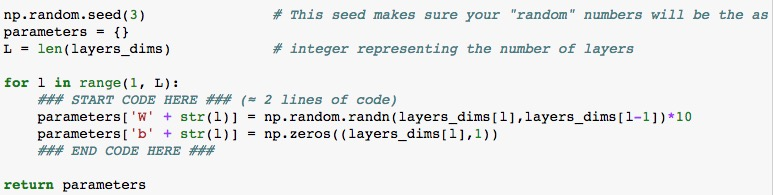
\includegraphics[width=10cm]  {15.jpg}}
 \caption{随机初始化}
  \label{fig:15}
 \end{figure}

 分析:

 起始的代价函数很大,这是由于我们采用的随机初始化的权重矩阵值较大,导致有些样本对于激活函数(sigmoid,输出层)输出结果值很靠近0或者1。
 当输出的结果值不同于真实值,其代价很大,比如$log(a^{[3]})=log(0)$,其代价是无穷大的。

过大或者过小的权重矩阵将导致梯度的暴涨或者快速衰减,这都会减缓优化算法获取最优结果的速度。为此,我们需要控制随机化的权重矩阵大小。

\subsubsection{He initialization He 初始化}
 He初始化方式(He et al., 2015.)正是为解决上面问题而提出的。
 这种初始化方式是对随机初始化的权重矩阵乘以sqrt(2./layers\_dims[l-1]))。
 另一种相识的初始化方式Xavier 方式,是对权重矩阵乘以sqrt(1./layers\_dims[l-1])。
 \begin{figure}[htb]
  \center{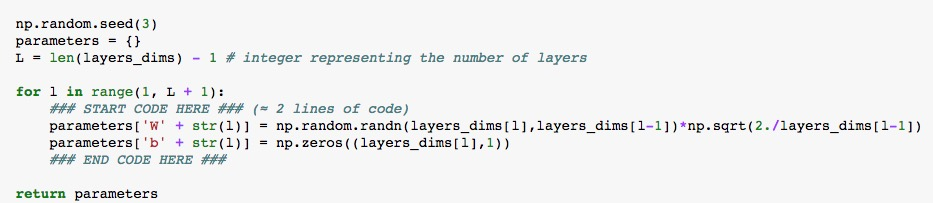
\includegraphics[width=10cm]  {16.jpg}}
  \caption{He 初始化}
   \label{fig:16}
  \end{figure}

总结:
\begin{figure}[htb]
 \center{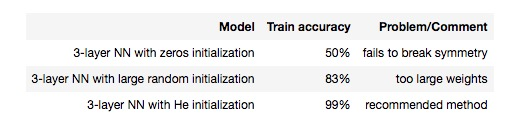
\includegraphics[width=10cm]  {17.jpg}}
 \caption{总结}
  \label{fig:17}
 \end{figure}

 \subsection{Regularization 正则化}
 对于L2正则化模型,需要用到的参数是lambd值。该正则化模型需要用到compute\_cost\_with\_regularization()
 和backward\_propagation\_with\_regularization()。

 而对于dropout模型则需要设置keep\_prob值作为神经元节点的概率开关。需要用到的函数是forward\_propagation\_with\_dropout()
 和backward\_propagation\_with\_dropout()。

 \begin{figure}[htb]
  \center{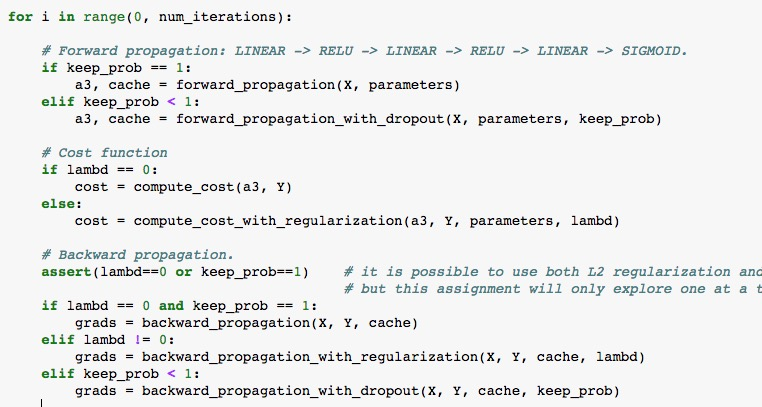
\includegraphics[width=12cm]  {18.jpg}}
  \caption{正则化}
   \label{fig:18}
  \end{figure}

存在过拟合。

\subsubsection{L2 Regularization}
公式:
\begin{figure}[htb]
 \center{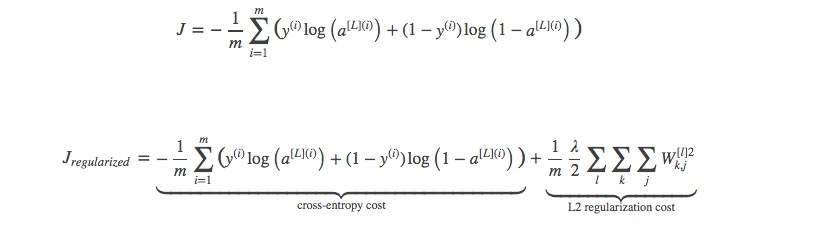
\includegraphics[width=12cm]  {19.jpg}}
 \caption{表达式}
  \label{fig:19}
 \end{figure}

 定义 compute\_cost\_with\_regularization()函数表示公式(2)的代价函数。
 $\sum_{k}\sum_{j}W_{k,j}^{[l]2}$的计算,我们可以采用 :np.sum(np.square(Wl))

由于我们有三个W参数 $W^{[1]}, W^{[2]} and W^{[3]}$, 所以需要将其分别计算,求和,再乘以 $(1/m)*(\lambda/2)$。
\begin{figure}[htb]
 \center{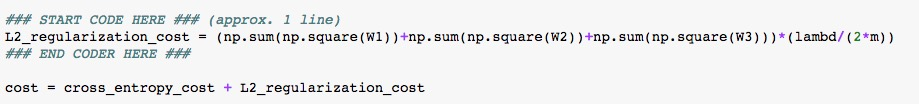
\includegraphics[width=12cm]  {20.jpg}}
 \caption{L2}
  \label{fig:20}
 \end{figure}

由于我们修改了代价函数,所以后向传播也需要做修改。同理,我们也仅仅需要修改dW1, dW2 and dW3。
对于这三者,每一项都需要加入正则项的梯度$\frac{d}{dW}(\frac{1}{2}\frac{\lambda}{m}W^2)=\frac{\lambda}{m}W$。

\begin{figure}[htb]
 \center{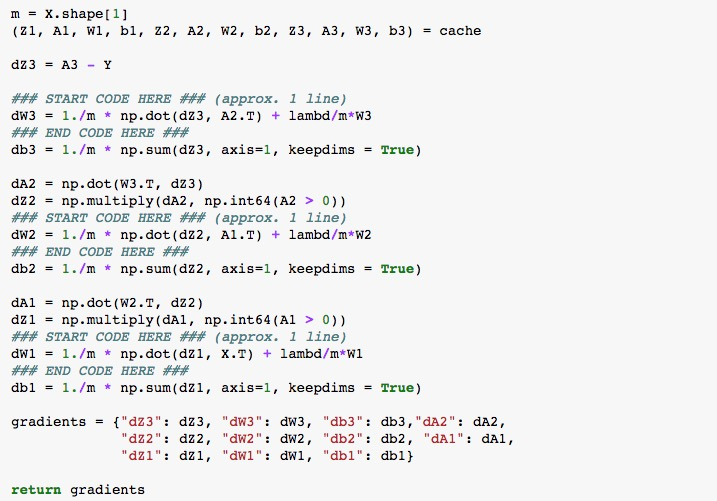
\includegraphics[width=12cm]  {21.jpg}}
 \caption{L2}
  \label{fig:21}
 \end{figure}

设置$\lambda$的值:parameters = model(train\_X, train\_Y, lambd = 0.7)

 讨论:

$\lambda$的值是可以通过对dev set的调整获取最优值。L2正则使得边界更加平滑,但是如果$\lambda$过大,会产生过度平滑,退化成一个线性回归,从而带来高偏差问题。
 L2正则化是基于较小的权值比较大的权值模型更简单这一假设。通过正则化,我们在代价函数中引入权重的平方值,这导致在反向传播时候,权重变得更小。

\subsubsection{Dropout Regularization}
dropout正则的前向传播:

$d^{[1]}$ 和 $a^{[1]}$ 尺寸一致,所以np.random.rand() 进行向量的初始化。对于矩阵 $D^{[1]}=[d^{[1](1)}d^{[1](2)}...d^{[1](m)}]$尺寸
和$A^{[1]}$一致,初始化方式类似。

根据keep\_prob对$D^{[1]}$矩阵做0-1划分。方式如 X = (X < 0.5),其实这是产生一个0-1矩阵mask,用于神经元节点的筛选。
$A^{[1]}$ to $A^{[1]}$∗$D^{[1]}$ 进行神经元节点的筛选操作。$A^{[1]}$ /keep\_prob,使得前后的期望值一致(inverted dropout)
\begin{figure}[htb]
 \center{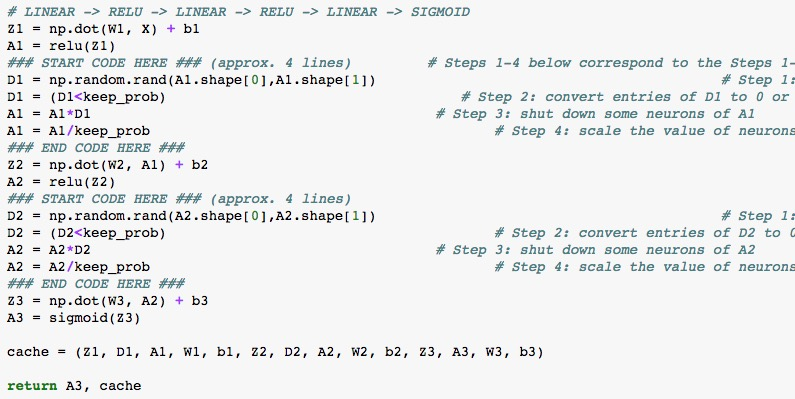
\includegraphics[width=12cm]  {22.jpg}}
 \caption{dropout 正则化前向传播}
  \label{fig:22}
 \end{figure}

dropout正则的后向传播:

前向传播过程中A1用到的$D^{[1]}$,在后向传播过程将$D^{[1]}$应用到 dA1即可。前向传播过程 将A1除以 keep\_prob ,以保持期望值。
在后向传播过程dA1也做如此操作,即 dA1 / keep\_prob 。这是由于$ A^{[1]}$被keep\_prob进行一定程度放大,则 其导数$ A^{[1]}$也需要做同比例的操作。
\begin{figure}[htb]
 \center{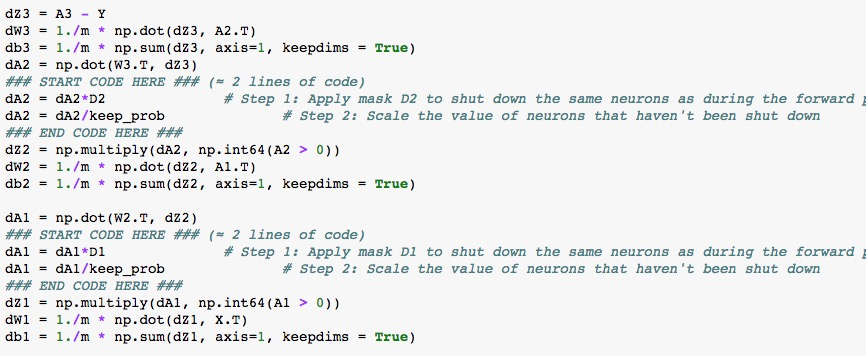
\includegraphics[width=12cm]  {23.jpg}}
 \caption{dropout 正则化后向传播}
  \label{fig:23}
 \end{figure}

 讨论:

 一个常见的错误是,将dropout同时用于训练集和测试集,记住一点:dropout仅仅用于训练集!

结论:
\begin{figure}[htb]
 \center{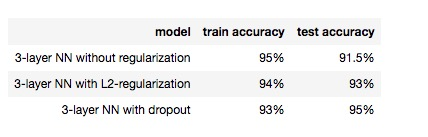
\includegraphics[width=12cm]  {24.jpg}}
 \caption{结论}
  \label{fig:24}
 \end{figure}

\subsection{Gradient Checking}
在神经网络计算过程中,对后向传播的梯度进行校验,确保其计算无误。至于,前向传播,由于相对简单,
所以,一般不会出错,在前向传播的基础上利用计算出来的代价J我们可以进行后向梯度的校验。

\subsubsection{1-dimensional gradient checking 一维梯度校验}
计算梯度近似值``gradapprox'': $gradapprox=\frac{J^{+}-J^{-}}{2\xi }$

计算两者difference:$difference=\frac{||grad-gradapprox||_{2}}{||grad||_{2}+||gradapprox||_{2}}$

范数的计算可以用np.linalg.norm(...)。当difference 足够小($<10^{−7}$),则可以视为梯度校验通过。
\begin{figure}[htb]
 \center{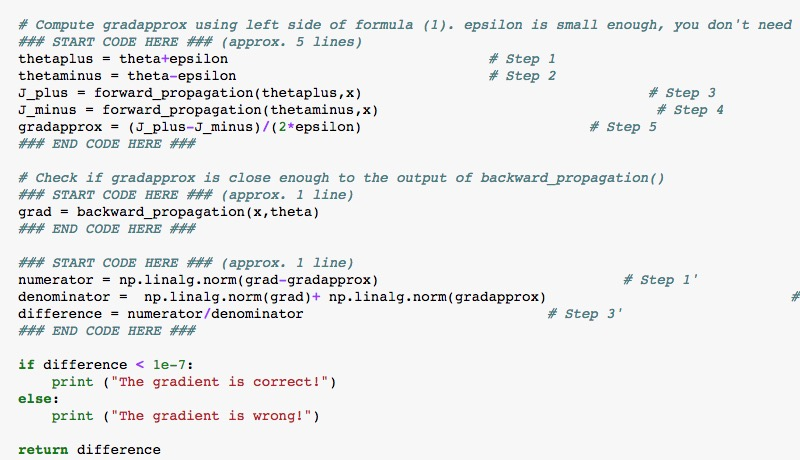
\includegraphics[width=12cm]  {25.jpg}}
 \caption{一维梯度校验}
  \label{fig:25}
 \end{figure}

\subsubsection{N-dimensional gradient checking n维梯度校验}

\begin{figure}[htb]
 \center{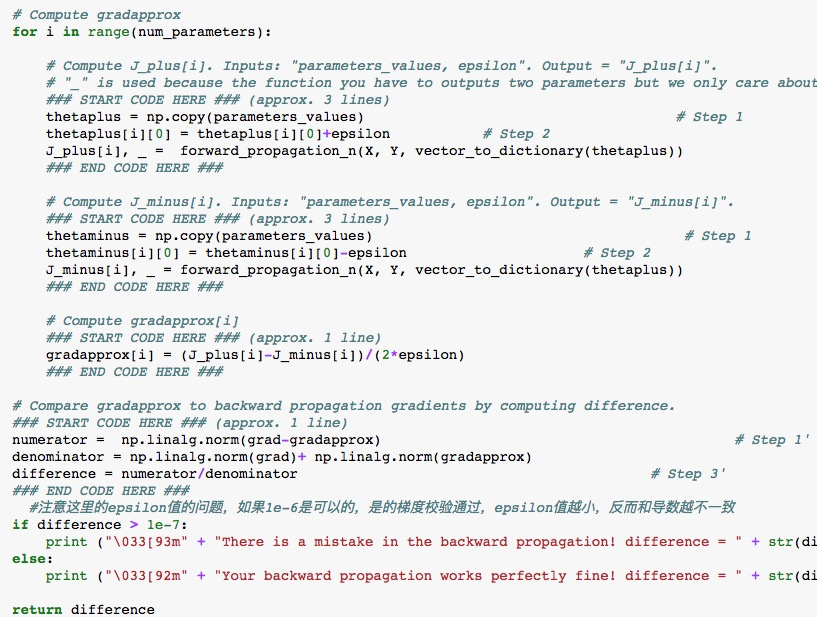
\includegraphics[width=12cm]  {26.jpg}}
 \caption{n维梯度校验}
  \label{fig:26}
 \end{figure}

所以,要注意看difference值是否和阈值相距很大。
本文为何就差那么一些,导致需要修改epsilon,可能是由于代价函数在局部存在毛刺,导致估算值和后向梯度计算结果,存在超于阈值的偏差。另外,relu的导数在0处有歧义,也可能导致此处的不够准确。

\subsection{Optimization Methods }
\subsubsection{Gradient Descent 梯度下降法}
梯度下降是每次处理完m个样本后对参数进行一次更新操作,也叫做Batch Gradient Descent。对于
L层模型,梯度下降法对于各层参数的更新:l=1,...L。
  \begin{equation*}
    W^{[l]}=W^{[l]}-\alpha dW^{[l]}
  \end{equation*}
\begin{equation*}
    b^{[l]}=b^{[l]}-\alpha db^{[l]}
\end{equation*}

update\_parameters\_with\_gd:
\begin{figure}[htb]
 \center{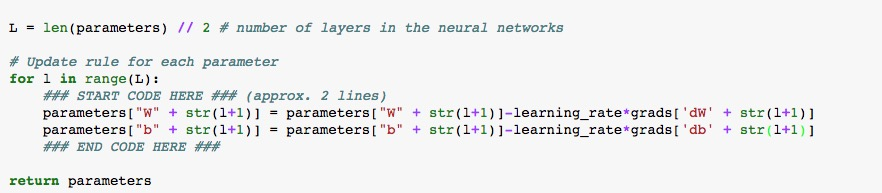
\includegraphics[width=12cm]  {27.jpg}}
 \caption{Gradient Descent}
  \label{fig:27}
 \end{figure}

Stochastic Gradient Descent (SGD) 随机梯度下降法。这等同于mini-batch中每个mini-batch只有一个样本的梯度下降法。此时,梯度下降的更新法则就变成,每个样本都要计算一次,而不是此前的对整个样本集计算一次。
\begin{figure}[htb]
 \center{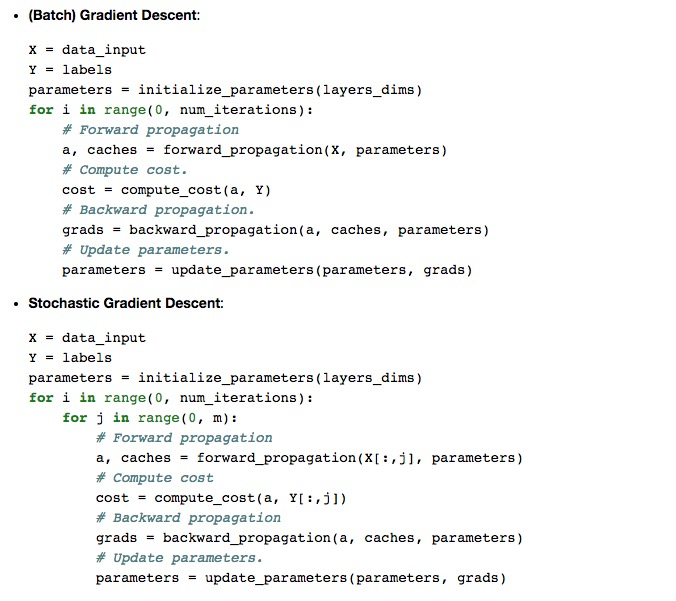
\includegraphics[width=12cm]  {28.jpg}}
 \caption{SGD vs GD}
  \label{fig:28}
 \end{figure}

当训练集很大时,这种方法可以明显提高运行速度,但是参数会沿着最小方向震荡,而不是平滑地收敛。

注意SGD共需要三个循环:
\begin{itemize}
  \item 最外层的迭代次数
  \item m个训练样本
  \item 每层参数的更新$((W^{[l]},b^{[l]})to(W^{[L]},b^{[L]}))$
\end{itemize}

谨记:
\begin{itemize}
  \item gradient descent, mini-batch gradient descent 和 stochastic gradient descent之间的区别在于梯度更新所用到的样本数据量。
\item 超参数学习率 α是需要调整获取到
\item mini-batch的尺寸也是调整获取到的,所以也是一个超参数。一般情况下这种方式比另外两者更好,特别是当训练集特别大的时候。
\end{itemize}

\subsubsection{Mini-Batch 梯度下降}
There are two steps:
\begin{itemize}
  \item Shuffle(洗牌)X和Y的随机要一致,否则Y值不能与X匹配
  \item Partition(分割) 尾部的数据可能小于一个mini\_batch\_size,所以对于最后一个mini-batch要注意处理。
\end{itemize}

当样本数无法被mini\_batch\_size整除的时候,最后一个mini-batch<mini\_batch\_size=64。[s]表示s向下取整(Python中实现:
math.floor(s))。

最后一个min-batch中样本数量= (m−mini\_batch\_size×⌊m/mini\_batch\_size⌋)。
\begin{figure}[htb]
 \center{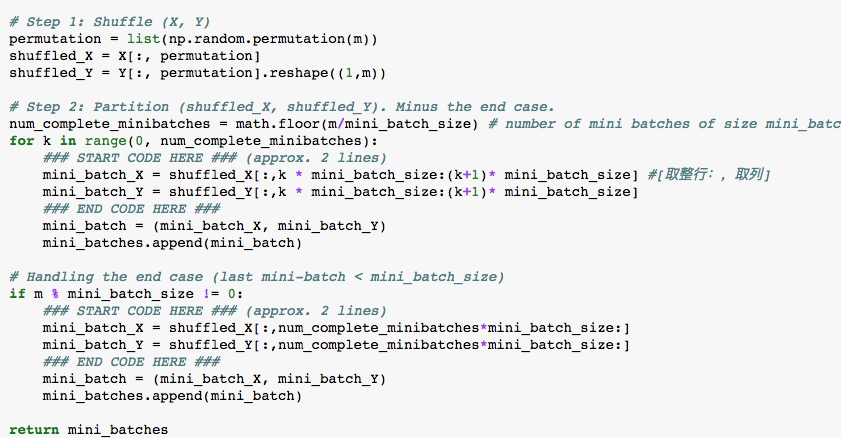
\includegraphics[width=12cm]  {29.jpg}}
 \caption{Mini-Batch}
  \label{fig:29}
 \end{figure}

一般mini-batch size的取值是$2^n$,如 16, 32, 64, 128等。
\subsubsection{Momentum 动量梯度下降法}
由于min-batch梯度下降法是在看过训练集的一部分子数据集之后,就开始了参数的更新,那么就会在参数更新过程中出现偏差震荡。
采用动量梯度下降法可以减缓震荡的出现。
momentum方式是在参数更新时候,参考历史的参数值,以平滑参数的更新。

velocity值初始化:initialize\_velocity 在Python中是一个字典,初始为0矩阵,其尺寸与 grads 一致。

带momentum的参数更新,l从1开始。:
\begin{figure}[htb]
 \center{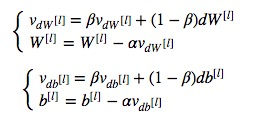
\includegraphics[width=8cm]  {30.jpg}}
 \caption{参数更新}
  \label{fig:30}
 \end{figure}

update\_parameters\_with\_momentum

注意:

velocity初始化为zeros,所以算法需要迭代一定次数以建立起速度,实现每次迭代的bigger steps。
当$\beta=0$,则退化成标准的梯度下降法。

$\beta$值的选取:

 越大,历史梯度值引入到当前值的权重越大,更新就会越平滑。但是如果太大,则会导致更新平滑过度。一般取值在0.8 到 0.999之间,常取0.9。
 可以通过尝试几个$\beta$值,然后看哪个值在降低cost function J效果最好,来获取最优值。

\subsubsection{Adam 算法}

\begin{figure}[htb]
 \center{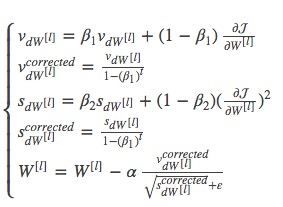
\includegraphics[width=7cm]  {31.jpg}}
 \caption{公式}
  \label{fig:31}
 \end{figure}

过程
\begin{figure}[htb]
 \center{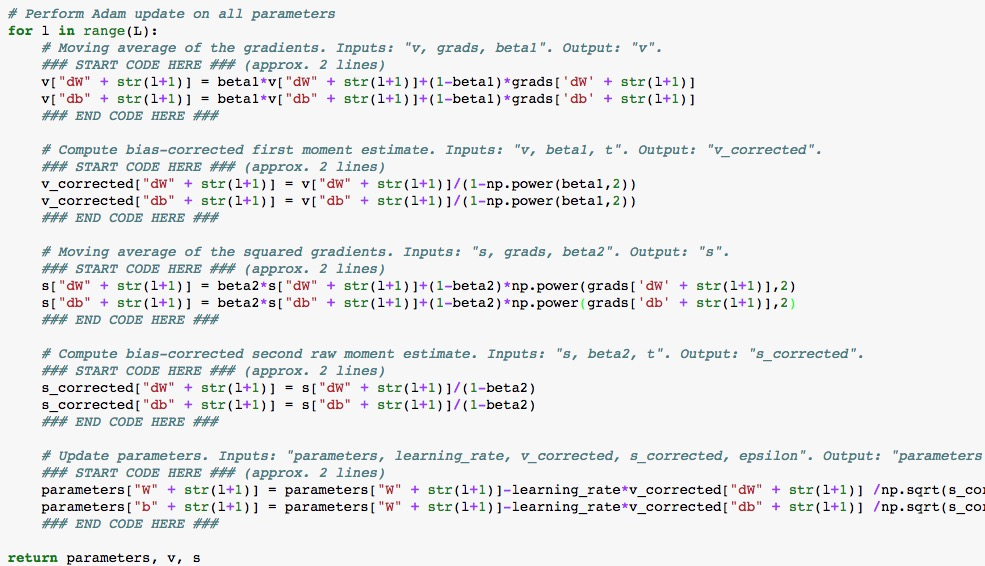
\includegraphics[width=12cm]  {32.jpg}}
 \caption{公式}
  \label{fig:32}
 \end{figure}

\subsubsection{总结}
Momentum一般都是有助于提升速度,但是当学习率较小,数据集相对简单的时候,其性能的优越性没有太明显。
我们在优化算法中看到的那些较大的震荡是由于一些minibatches 相对更加复杂所造成的。

从运行结果可以看出,Adam算法比mini-batch gradient descent 和 Momentum都要显得优越。
对于model如果在简单数据集上,迭代次数更多的话,这三种优化算法都会产生较好的结果,但是我们也可以看出,Adam算法收敛得更快些。

Adam算法的优点::

内存要求低 (尽管比gradient descent 和 gradient descent with momentum要高些)
一般微调超参数就可以获得较好的结果(除了$\alpha$)

\begin{figure}[htb]
 \center{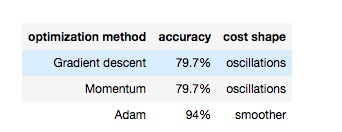
\includegraphics[width=8cm]  {33.jpg}}
 \caption{结论}
  \label{fig:33}
 \end{figure}

\end{document}
